\section{Introduction}
\label{sec:intro}



\begin{figure}[!t]
\centering
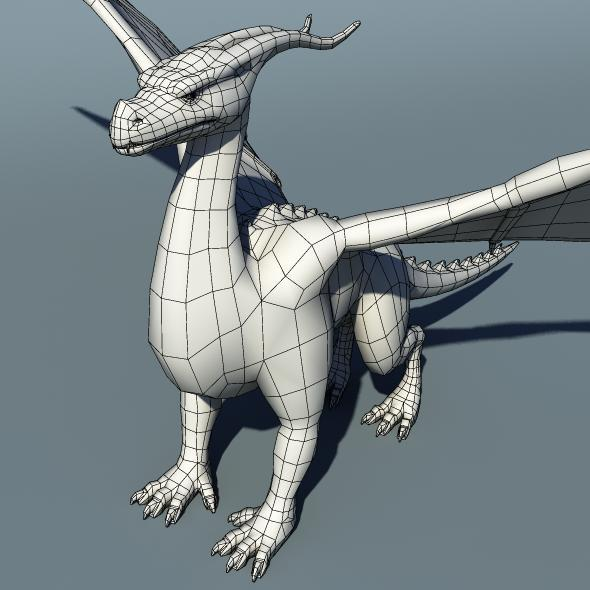
\includegraphics[width=2.5in]{dragon}
\caption{A mesh graph where lines correspond to edges and intersections of lines correspond to vertices.}
\label{fig:mesh}
\end{figure}

\subheading{Contributions}

We anticipate contributing a new technique for and a well-engineered
implementation of a cache-efficient data-graph computation using
priority-dag scheduling.  In addition, our implementation will support
extremely large simulations on distributed-memory clusters.  Both
of these contributions are high-impact features for the customers
of Simit, for which \proc{Prism} will be the new backend for multi-cores
and clusters of multi-cores.  We have some initial exploratory code
of priority functions (e.g. BFS depth, color).  

\subheading{Task Breakdown}

James and Predrag will extend \proc{Prism} to support data reshuffling
based on a priority per vertex.  Initially, this will be a standalone
utility that reads a graph file, reorders the vertices and writes out
the shuffled file.  

Will and Mohsen will engineer the MPI support for distributed memory,
including support for distributed data loading.

\subheading{Issues}

We descoped our project to focus on being a good back-end for Simit, which
works on graphs of physical simulations.  This means ditching the investigation
of software prefetching and static assignment of vertices to processors.
However, our new focus has allowed us to do something more elegant, essentially
a cache-oblivious scheduling algorithm for data-graph computations on graphs
of physical simulations.

\section{Introduction}
\label{sec:intro}

This section introduces the problem of deterministically scheduling data-graph
computations while preserving good cache efficiency on the special subset of graphs
that are locally connected and embeddable in a low-dimensional space.  

\subsection{Cache Efficiency Perils}

This section will demonstrate the cache efficiency issues inherent in chromatic
scheduling and dag-scheduling with a poor priority function.  

\subsection{Distributed Memory}

In this section, we will discuss
the challenges in extending the implementation of \proc{Prism} to support
distributed memory. 
